\documentclass[rinkou,a4paper]{ieicej}
% \usepackage{graphicx}
\usepackage[dvipdfmx]{graphicx}
\usepackage{url}
\usepackage{paralist}
\usepackage{nidanfloat}
\usepackage{ascmac}
\usepackage{fancybox}
\usepackage{amsmath}
\usepackage{amssymb}
\usepackage{amsfonts}
\usepackage{pifont}
\usepackage{multirow}
\usepackage{comment}

% UserSetting
\newenvironment{narrow}{\baselineskip=3mm}

\setcounter{page}{1}
\vol{103}%year
\no{04}%month
\day{17}%day

\jtitle{HTTP通信におけるIPv4とIPv6のネットワーク環境比較}%title
\jsubtitle
\authorlist{
 \authorentry{平野 紘大}{Kodai HIRANO}{}
} \vspace{-3mm}
\begin{document}

\maketitle

\section{はじめに}
インターネットの世界的な普及により,IPv4アドレスの国際的な在庫(IANA Pool)が,2011年2月3日に枯渇した.また,2011年4月15日には,アジア太平洋地域のRIR(APNIC)の在庫も枯渇した.

現在は,未使用アドレスの再利用や,NAPTなどによって対応している.アドレスの価格も上昇しており,インターネットの発展を妨げている.

この問題を解決するためには,IPv4の後継規格であるIPv6を推進することが必要である.現状のIPv4でのネットワーク環境を,IPv6で引き継ぐためには,IPv4と同等以上の性能が求められる.

本研究では,IPv6ネットワークの現状を把握するため,IPv4との通信品質の比較という観点でのネットワーク計測を実施する.

\section{既存研究}
\subsection{RTTによる比較}
\cite{kitaguchi1}で北口らは,同一クライアントからの,IPv4とIPv6によるHTTP通信を比較し,ネットワーク品質を評価している.

TCPコネクションの確立時に送受信される,SYN+ACKパケットとACKパケットの応答時間(RTT)によって,サーバ・クライアント間のネットワーク通信遅延を求めている.

2009年6月から2010年6月までの,1年間のデータを分析している.IPv4アドレスを基に,ユーザを特定し,ユーザ毎の通信遅延の中央値を算出して,用いている.地域毎の,IPv6トンネル接続とネイティブ接続の比率の推移も示している.地域毎に,IPv4とIPv6のRTTの比率の推移を示している.日本にサーバーを設置したため,ARIN地域(北アメリカ)やRIPE地域(ヨーロッパ,中東,中央アジア)では,オーバーヘッドが大きく,IPv4とIPv6の遅延差が評価しにくいため,APNIC地域(アジア,太平洋地域)のユーザーに焦点を当てて,分析している.

IPv6の通信遅延は,ネイティブ接続はトンネル接続に比べると,IPv4に近い品質であるものの,IPv6の遅延が大きいという調査結果となっている.

\subsection{MSSとTTLによるネットワークの推定}
\cite{kitaguchi2}で北口らは,HTTP通信の観測によって,IPv4とIPv6のネットワーク環境の比較をしている.

TCPでのMSS(Max Segment Size)値と,IPにおけるTTL(Time To Live)値(IPv6の場合にはHop Limit値)で,通信路とホップ数を推定し,IPv6ネットワークの展開状況を,推測している.

MSSは,TCP通信で送受信できる,最大のパケット長である.このMSSは,TCP通信の開始時に,ユーザー側が,サーバー側に対して宣言するもので,MSS値を観測することで,通信路がどのようなものかを推測することができる.MSS値により,ヘッダの長さを求めて,通信路の形態(PPPoEなど)を推測する.

TTLは,IPヘッダに設定されている値で,パケットがルータを経由できる最大値を示す.ルータを経由するたびに,1ずつ減算されるので,デフォルト値とサーバー到着時の値を用いて,ホップ数を割り出している.

地域毎の通信路の特徴を分析している.IPv4とIPv6のホップ数を比較することで,トポロジがどれくらい違うのかを推測している.

\subsection{先行研究との違い}
\cite{kitaguchi2}では,ネットワーク環境を推定するにとどまっているので,ネットワーク環境の推定手法を借りて,品質の比較まで行う.また,\cite{kitaguchi1}では,通信遅延のみを品質として評価していたが,帯域幅も計測し,評価する.

\section{計測手法}
基本的には\cite{inonius}と同じ

HTTP GET/POSTによる通信を用いて計測

ダウンロードの速度計測

1MByteのデータを15秒間ダウンロードし続け、その際の帯域値を計測し平均値を求めます。200m秒毎に計算し、画面上のメーターに表示します。

アップロードの速度計測

HTTPのヘッダのみのデータを、HTTP POSTにより15秒間転送し続けて帯域値を計測し平均値を求めます。200m秒毎に計算し、画面上のメーターに表示します。

帯域幅を計測するために,10GのNICを用いて,サーバー側がボトルネックにならないようにする.

取得する情報:IPアドレス,時刻,Upload,Download,遅延,Jitter,位置情報

\begin{figure}[hh]
\centering
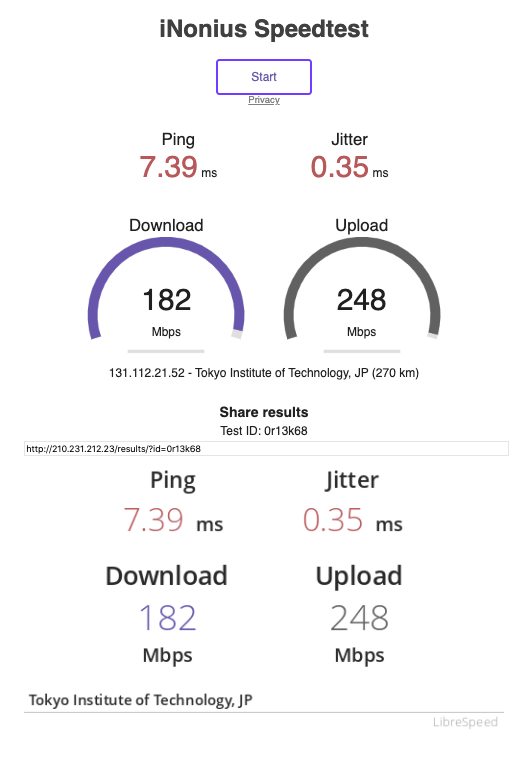
\includegraphics[scale = 0.4]{Screenshot.png}
\caption{現状のサイト(http://210.231.212.23/)}\label{ss}
\end{figure}

\begin{figure}[ht]
\centering
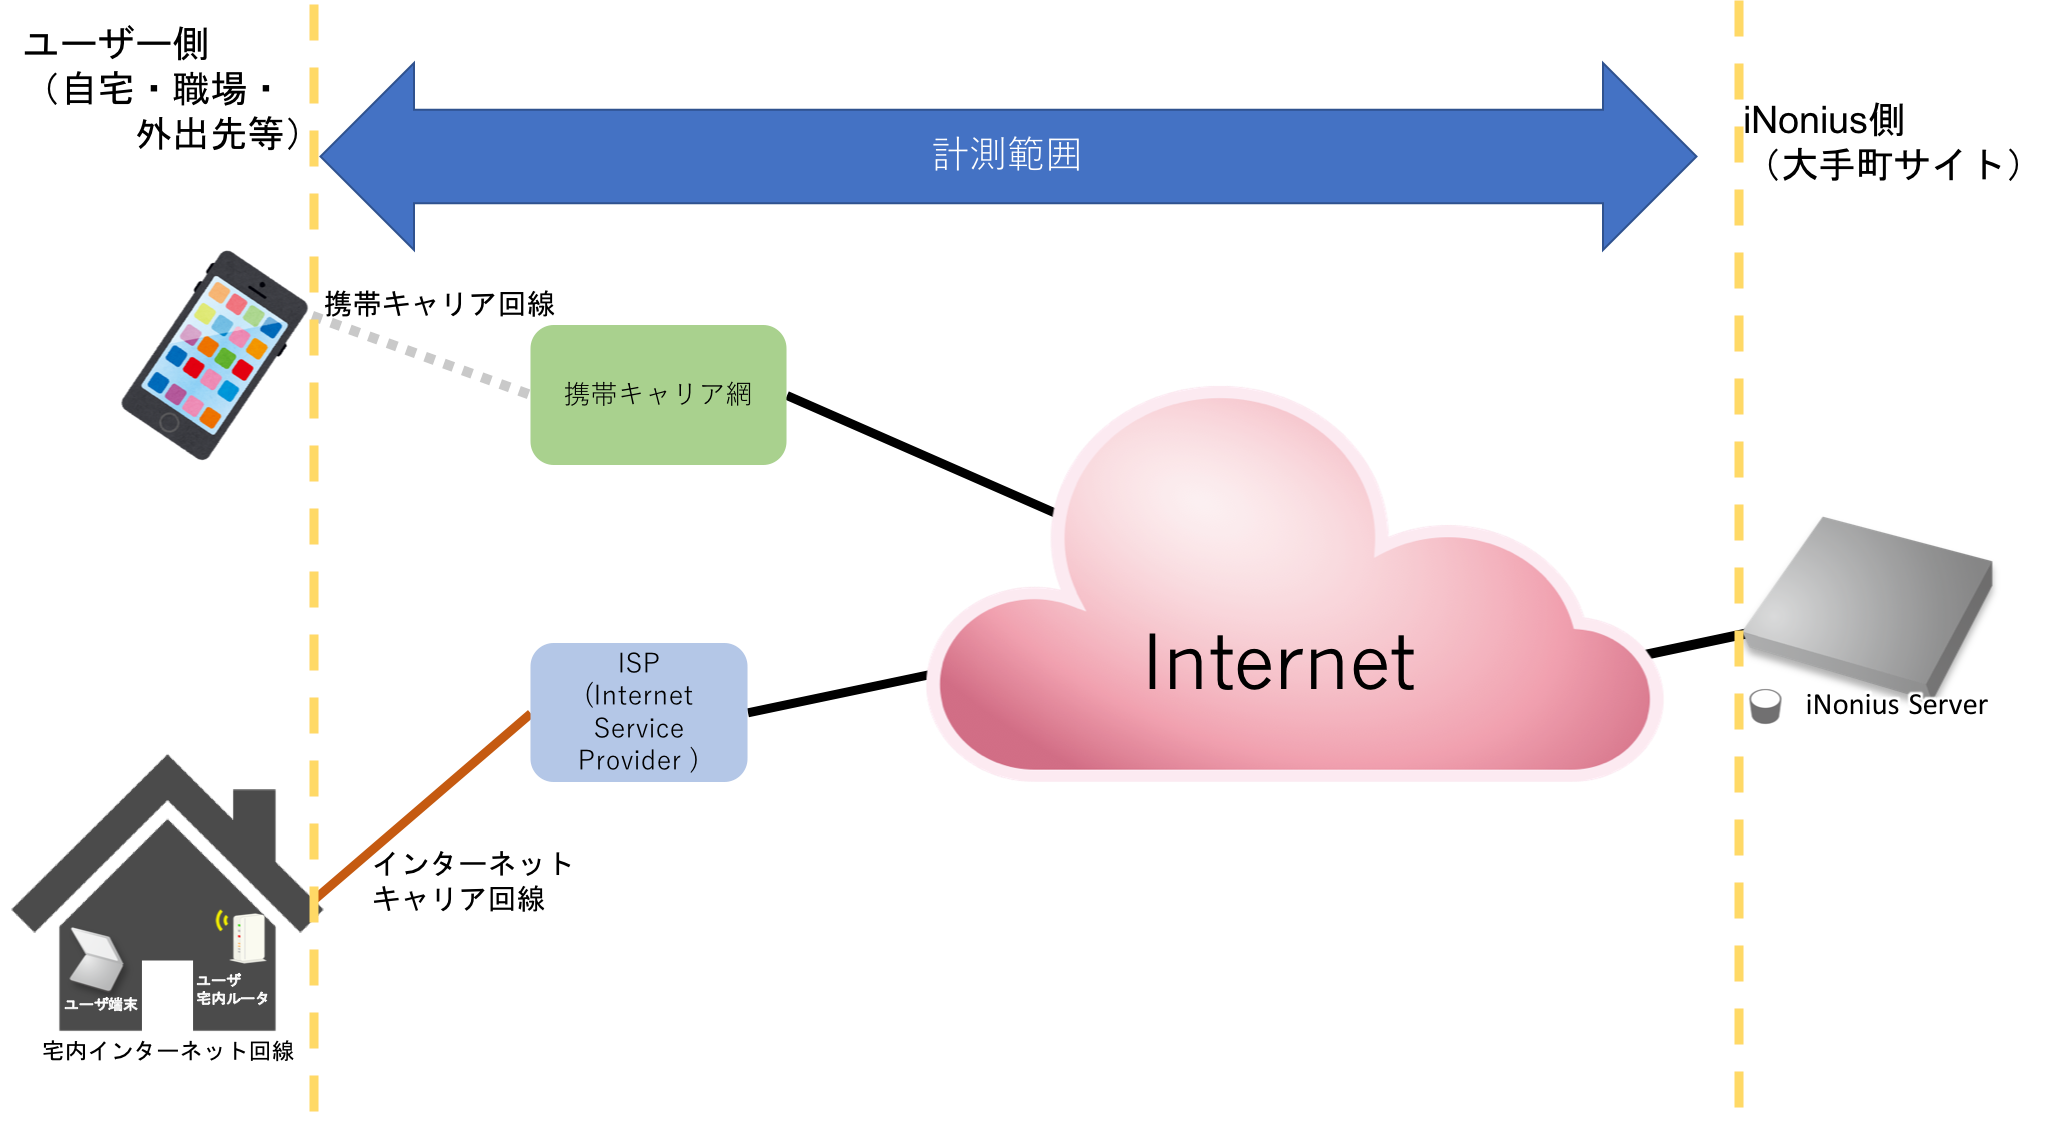
\includegraphics[scale = 0.25]{structure.png}
\caption{ネットワーク構成}\label{struct}
\end{figure}


\subsection{残タスク}
目標の計測までの残タスクをまとめる.
\subsubsection{デュアルスタック}
サーバーをIPv4とIPv6の両方に対応させる.IPv4/6の計測完了後,ユーザーのネットワークがIPv6/4に対応していた場合,自動的にIPv6/4での計測を始める.
\subsubsection{ユーザー同定}
本研究の目的は,IPv4とIPv6の通信状況の比較である.したがって,同一のユーザーからのIPv4とIPv6の通信を比較,評価する必要がある.
北口らの研究\cite{kitaguchi1}では,urlパラメータに,userIdを持たせて,同じユーザーからの通信を識別している.これは\cite{kitaguchi2}でも利用されている.

また,大量のアクセスが同じユーザー(ヘビーユーザー)からあった場合,その影響を考慮する必要があるので,IPv4 アドレス
を基にユーザを特定する.

また,Route Views Project\cite{routeview}が公開しているBGPのフルルート情報を用いて,AS情報を求めている.

\subsection{PPPoEやIPoEなど通信路の形態の推定}
\cite{kitaguchi1}では,AS番号がIPv4とIPv6で異なるとき
\begin{itemize}
 \item IPv4とIPv6でそれぞれ別のAS経由でネイティブ接続している
 \item IPv4 over IPv6(IPv6はネイティブ)
\end{itemize}
のパターンは少ないと仮定し,IPv6はトンネル接続として,AS番号が同じならば,IPv6はネイティブであるとしている.

\cite{kitaguchi2}では,MSS値により,ヘッダの長さを求めて,通信路を推定している.また,[1]での推定方法との比較をして,上記の仮定を否定している.

\subsubsection{UI/UX}

\section{計測結果の分析}






\begin{thebibliography}{9} % 文献数が10未満の時 {9}  文献数が10以上の時 {99}
\bibitem{kitaguchi1}
 北口 善明, 伊波 源太, 永見 健一,``HTTP通信からみたIPv4とIPv6通信遅延の比較評価'' ,IEICE Technical Report, IA2010-37(2010-9)
\bibitem{kitaguchi2}
 北口 善明, 伊波 源太, 永見 健一,``HTTP通信を利用したIPv4とIPv6のネットワーク環境比較'' ,IPSJ SIG Technical Report, vol.2011-IOT-12 No.16
\bibitem{routeview}
University of Oregon Route Views Project,http://www.routeviews.org/, January 2005.
\bibitem{inonius}
iNonius Project,https://inonius.net/

\end{thebibliography}

\end{document}
